
\begin{table}[h]
    \centering
        \caption{\textcolor{black}{95\% confidence interval of the solution obtained using different scenario sets for each number of scenarios.}}
        {\color{black}
        \begin{tabular}{c|c|c}
        \hline
             \makecell{Number of \\ scenarios} & 95\% CI (kW) & \makecell{Average objective \\ value (kW)} \\
        \hhline{===}
             $7$ & $\left[6105.95, 6393.99\right]$ & $6249.57$ \\
        \hline
            $21$ & $[3764.35, 4414.53]$ & $4089.44$ \\
        \hline
            $49$ & $[2596.13, 2842.21]$ & $2719.17$ \\
        \hline
            $98$ & $[2721.20, 2879.54]$ & $2800.37$ \\
        \hline
            $147$ & $[2705.10, 2823.21]$ & $2764.16$ \\
        \hline
        \end{tabular}}
        \label{tab:95_CI}
    \end{table}

\clearpage
% \newpage
%%%%%%%%%%%%%%%%%%%%%%%%%%%%%%% Spatiotemporal Impact Assessment Chapter %%%%%%%%%%%%%%%%%%%%%%%%%
\section{Spatiotemporal impact assessment of hurricanes and storm surges in electric power systems}
\subsection{Prior work on extreme weather impact assessment on power systems and their limitations}
Several existing works model the impacts of hurricanes on the power grid due to high-speed winds~\cite{7434044}. To model the spatial nature of the event, other works divided the entire power grid into zones such that each zone experiences a different wind speed~\cite{Trakas2018}. However, based on the hurricane's trajectory, each component is impacted differently as the hurricane moves inland, rendering the simplified hurricane model inaccurate for grid impact assessment. Other works model the effect of hurricanes on distribution grid~\cite{nguyen2019assessing}. Since the overall spatial exposure of a hurricane is greater than an entire distribution grid for each time step, the analysis based on the distribution system alone would not be meaningful enough.
Furthermore, none of these works model the impact of storm surges on the power grid. In~\cite{souto2022power}, a power system impact assessment framework is presented to identify potential mitigation strategies and enhance resilience against floods. A stochastic optimization framework for substation hardening against storm surge is presented in~\cite{shukla2021scenario}. \cite{Feng2022} evaluated the impacts of tropical cyclones and heatwaves on the power grid. The existing work, however, lacks the spatiotemporal impacts analysis of hurricanes characterizing the compound effects of high-speed wind and flooding. 

\subsection{Proposed Approach and Modeling}
This work aims to develop a compound spatiotemporal effect of hurricanes and storm surges on electric power systems. First, dynamic hurricane scenarios are generated based on historical hurricane tracks and storm surge scenarios are obtained based on the obtained hurricane parameters closer to the landfall. Next, sequential Monte Carlo simulation (MCS) is performed for probabilistic tracks and flooding scenarios for each time step as the hurricane moves inland. Finally, we quantify the impacts using a spatiotemporal loss metric based on the compound effect of hurricanes and floods.

\subsubsection{Hurricane Wind field Model}
A part of the impact of hurricanes originates from their wind speed. This wind speed is a vector field centered around the hurricane's eye and changes as it moves inland. This wind field can be modeled as an equation with three variables: $v_{max}$, $R_{v_{max}}$, and $R_s$~\cite{javanbakht2014risk, 9917119}. Here, $v_{max}$ measures the maximum sustained wind speed of the hurricane in knots, $R_{v_{max}}$ measures the distance to $v_{max}$ in nautical miles (nmi), and $R_s$ measures the radius of the hurricane from the hurricane's eye, also known as the radius of the outermost closest isobar (roci), in nmi. Fig.~\ref{fig:static_hurricane} demonstrates the relationship between the wind speed and the distance from the hurricane's eye, and the piecewise mathematical function that represents Fig.~\ref{fig:static_hurricane} is shown in (\ref{eq:static_eq}).

\begin{equation} \label{eq:static_eq}
\small
\begin{aligned}
&v(x)= \begin{dcases} K \times v_{max}(1-exp{[-\Psi x]}) & 0 \leq x<R_{v_{max}} \\
v_{max} \exp \left[- \Lambda \left(x-R_{v_{max}}\right)\right] & R_{v_{max}} \leq x \leq R_{s} \\
0 & x>R_{s}\end{dcases} \\
&\Psi=\frac{1}{R_{v_{max}}} \ln \left(\frac{K}{K-1}\right), K>1;
\quad \Lambda = \frac{\ln \beta}{R_{s}-R_{v_{max}}}
\end{aligned}
\end{equation}

\noindent
$K$ is a known hurricane constant, $x$ is the distance from the hurricane eye, and $\beta$ is the factor that the maximum sustained wind speed will decrease at the hurricane’s boundary $(R_s)$. Using this equation, it can be assumed that the hurricane has no effect outside this boundary.

\begin{figure}[t]
    \centering
    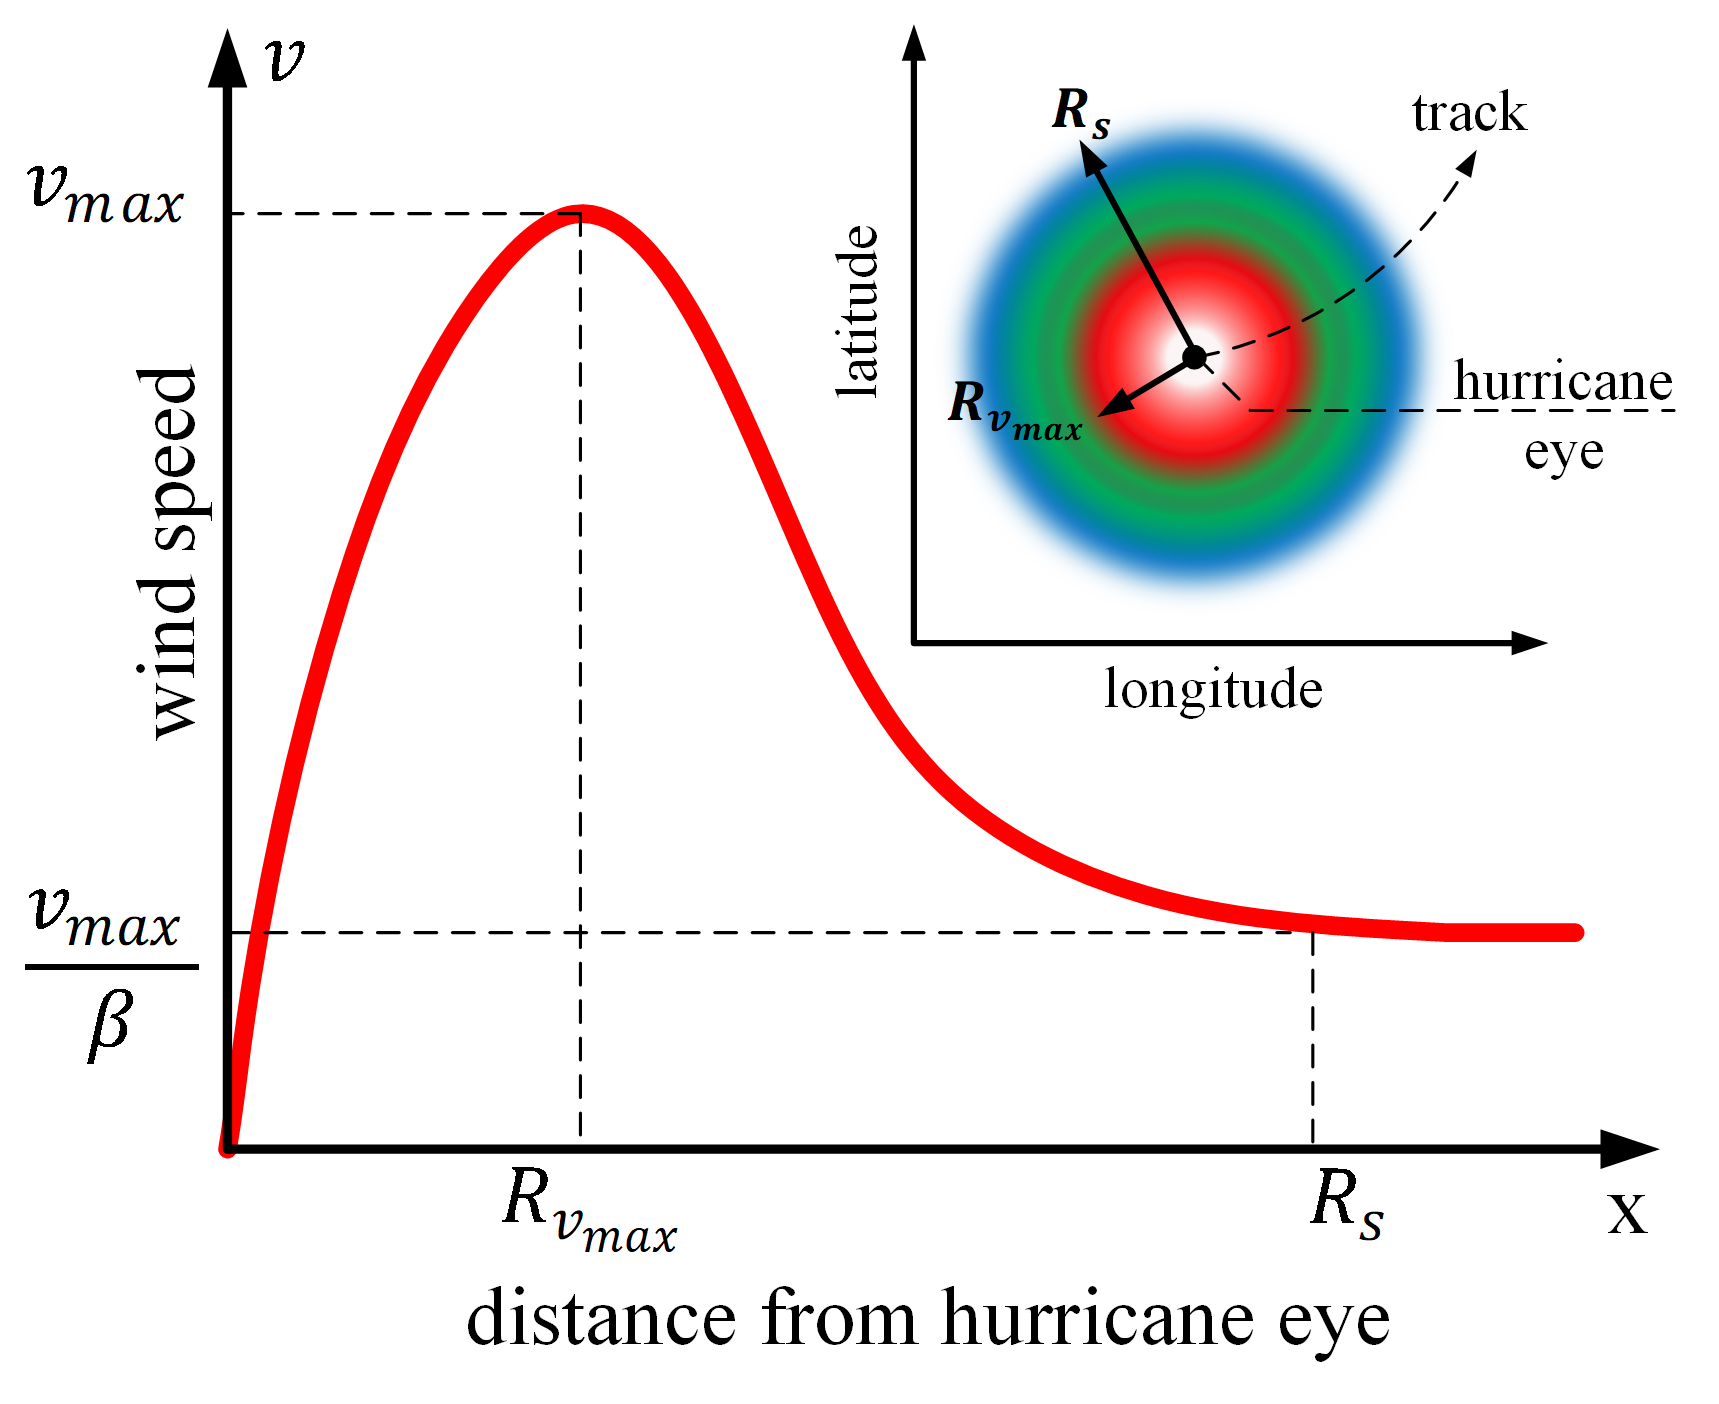
\includegraphics[width=0.55\textwidth]{figures/hurricane_wind_field.png}
    \caption{Static gradient wind field of a typical hurricane.}
    \label{fig:static_hurricane}
\end{figure}

To ensure a realistic hurricane wind field, the wind parameters in (\ref{eq:static_eq}) are obtained using the International Best Track Archive for Climate Stewardship (IBTrACS). IBTrACS is a global collection of tropical cyclones that merges data from multiple agencies to create a database for historical hurricane parameters at various time steps~\cite{Knapp2010}. The hurricane wind field is generated for each time step $t$ by obtaining $\{R_{v_{max}}^t$, $R_{s}^t$, $v_{max}^t\}$ from IBTrACS and using Eq. (\ref{eq:static_eq}). The problem of missing data is often possible when using historical data of higher resolution. IBTrACS, however, has approximated values of wind speed at each specified time interval. The work in~\cite{javanbakht2014risk} argues that the individual elements in $\{R_{v_{max}}^t$, $R_{s}^t$, $v_{max}^t\}$ are highly uncorrelated and hence one can randomly sample the corresponding element to approximate the behavior of the hurricane at that particular instance. Hence, for such situations, we have randomly sampled one of the parameters whenever required. The distribution of three of these parameters for historical hurricanes from 1851 -- 2012 is shown in Fig.~\ref{fig:three graphs}.       

\begin{figure}[ht]
    \centering
    \begin{subfigure}[t]{0.55\textwidth}
        \centering
        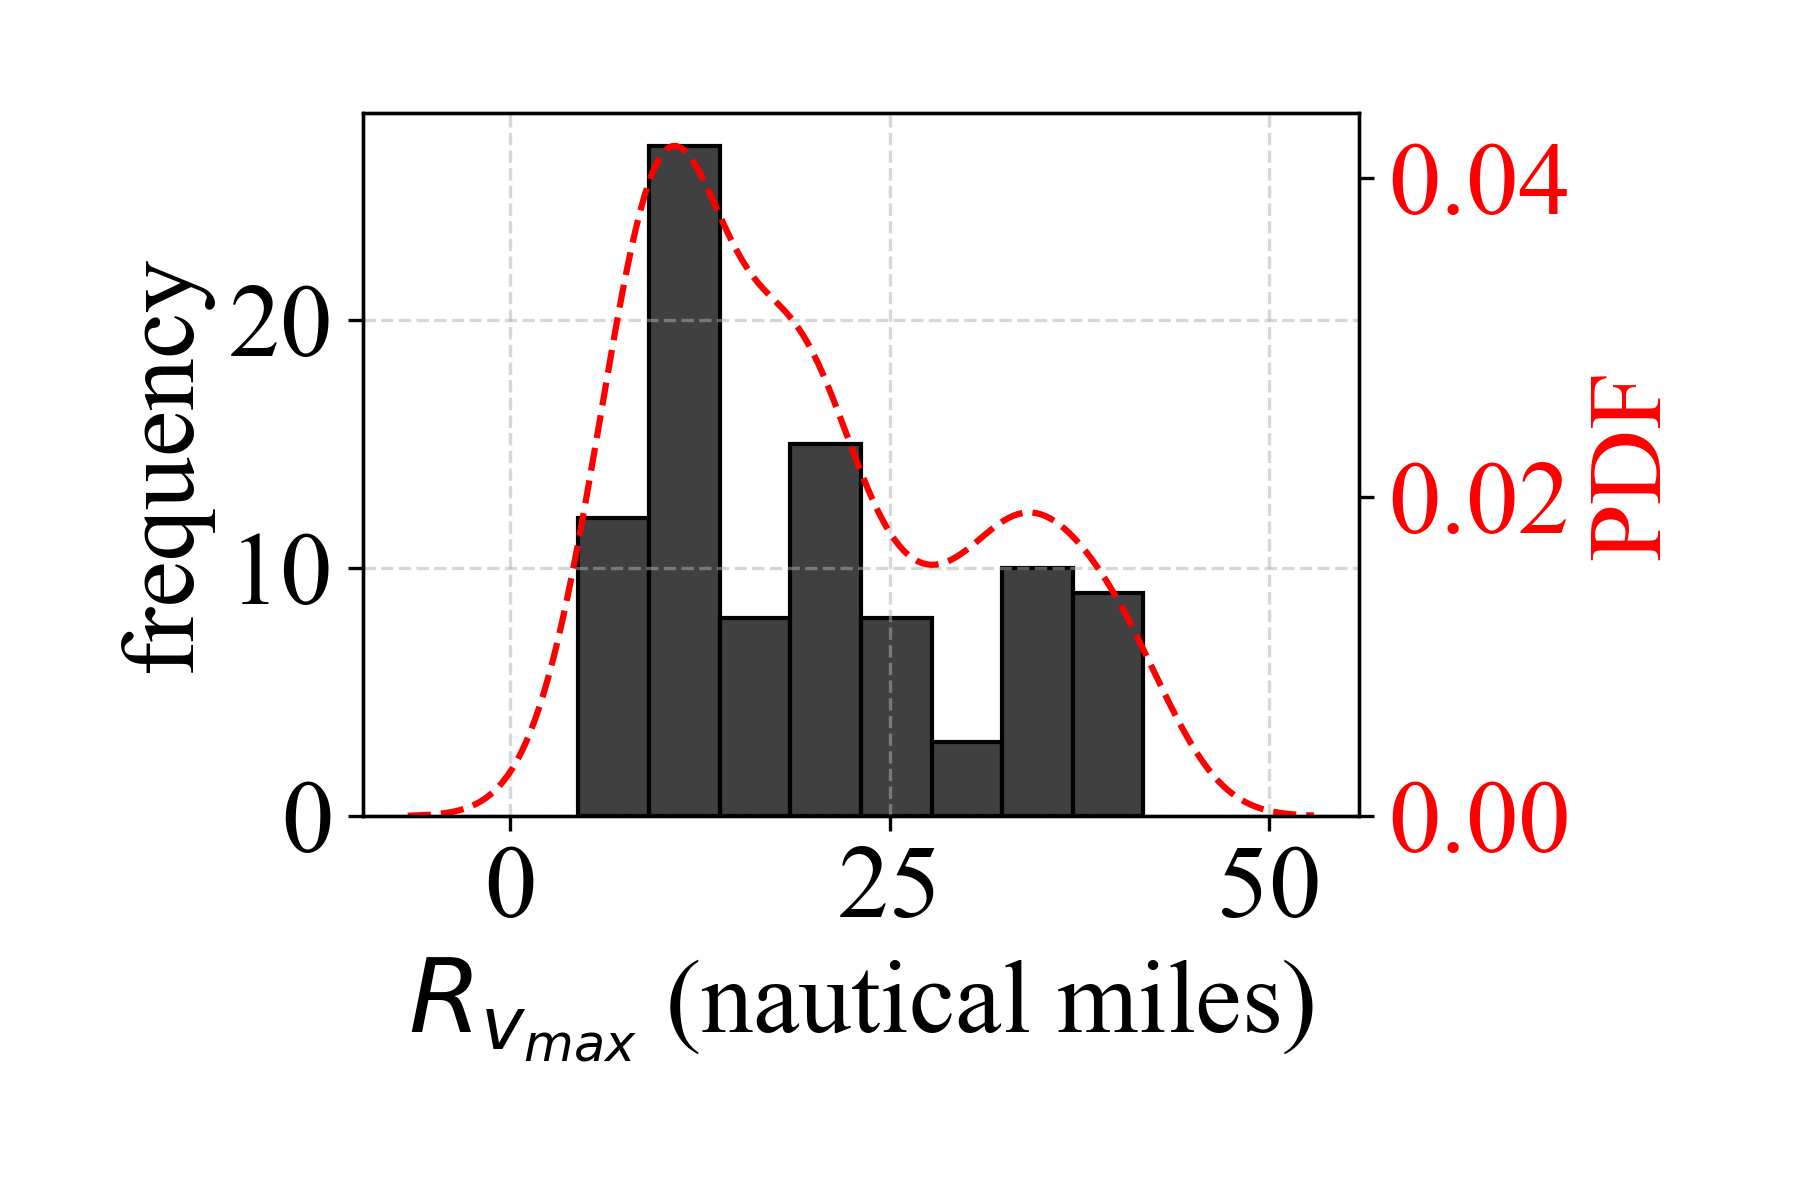
\includegraphics[clip, trim=0cm 0.7cm 0.1cm 0.5cm, width=\linewidth]{figures/Rmw_kde.png}
        \caption{}
        % \label{fig:MC_trial}
    \end{subfigure}%
    \hspace*{\fill}
    \begin{subfigure}[t]{0.55\textwidth}
        \centering
        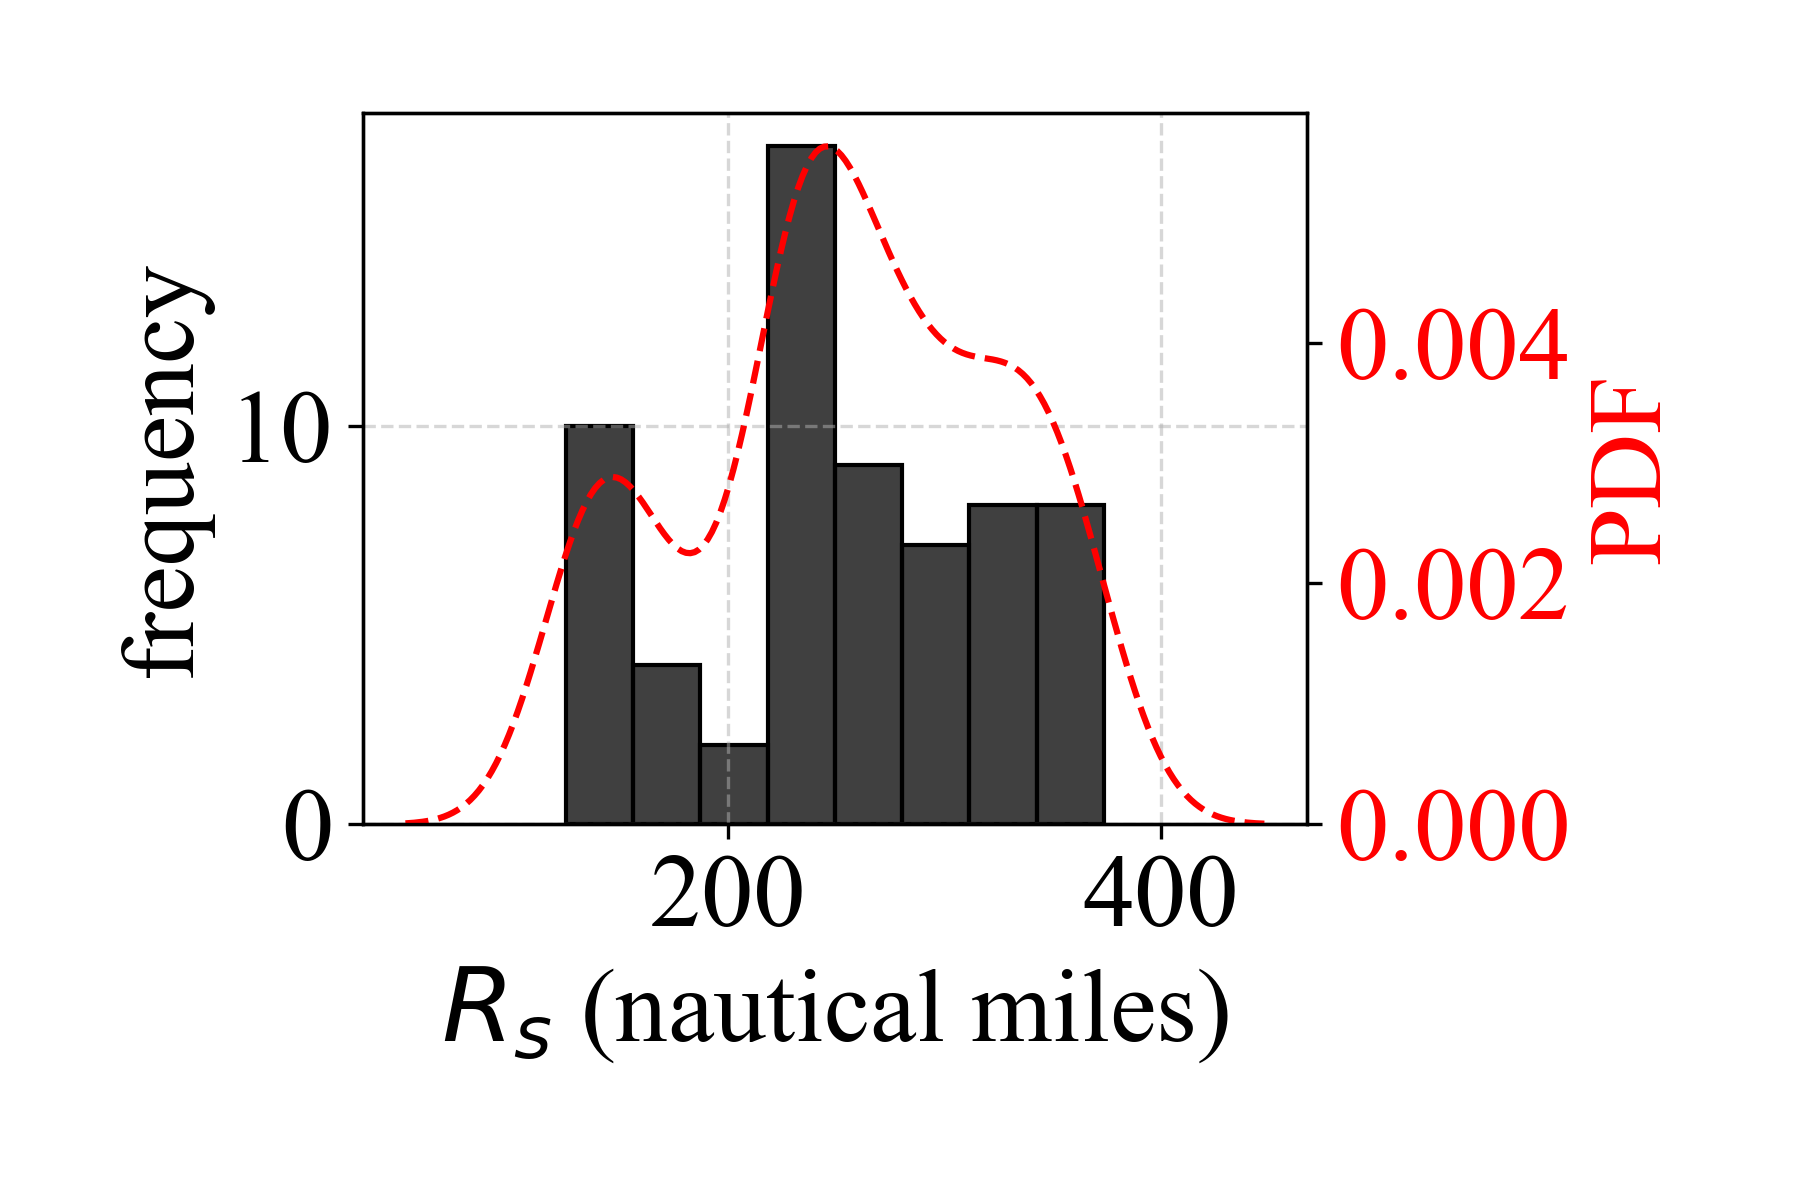
\includegraphics[clip, trim=0cm 0.7cm 0.1cm 0.5cm,width=\linewidth]{figures/Rs_kde.png}
        \caption{}
        % \label{fig:outage_prob}
    \end{subfigure}
    \bigskip
    \hspace*{\fill}
    \begin{subfigure}[t]{0.55\textwidth}
        \centering
        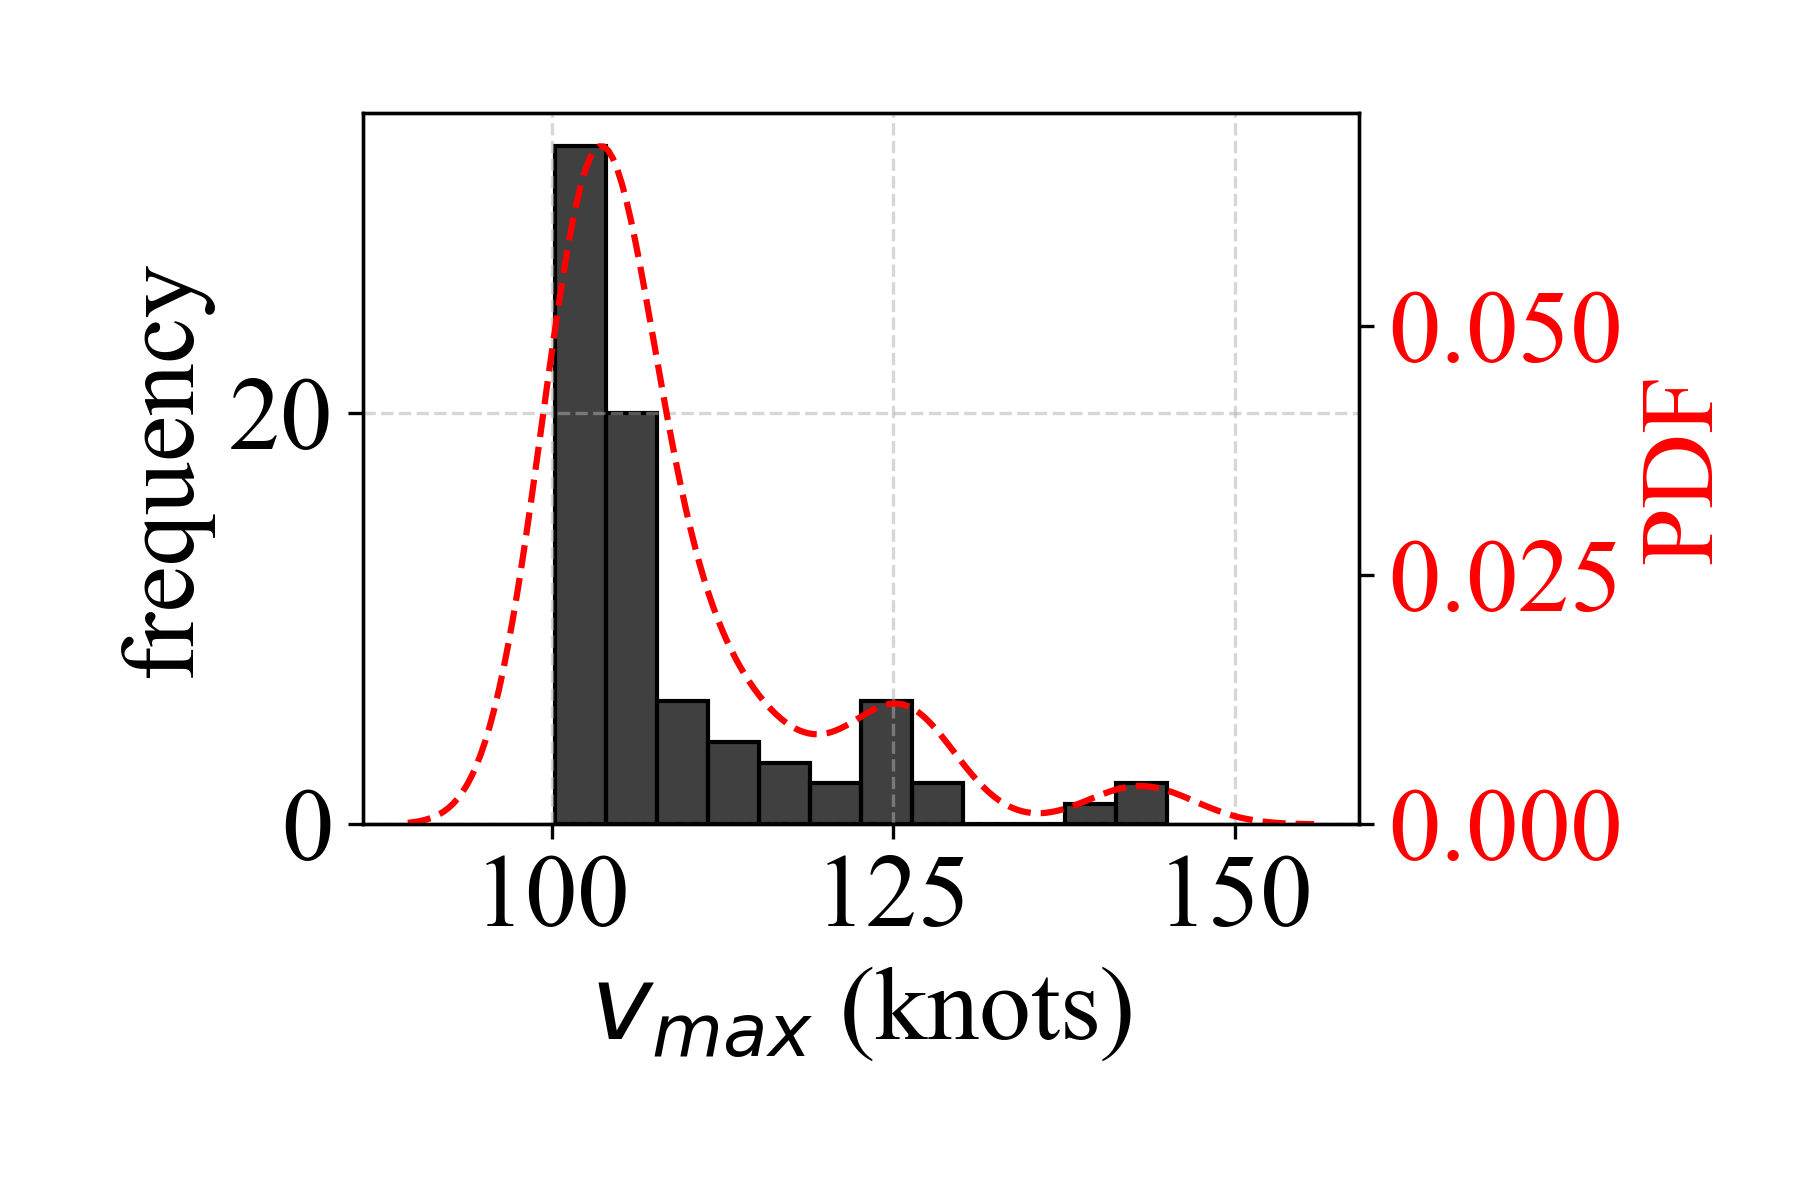
\includegraphics[clip, trim=0cm 0.7cm 0.1cm 0.5cm,width=\linewidth]{figures/Wm_kde.png}
        \caption{}
        % \label{fig:loss_scen}
    \end{subfigure}
    \hspace*{\fill}
    \vspace{-10pt}
    \caption{KDE of a) $R_{v_{max}}$, b) $R_s$, and c) $v_{max}$ estimated from the actual hurricanes that occurred in the USA~(1851--2012).} 
    \label{fig:three graphs}
\end{figure}

\subsubsection{Storm Surge Model}
In this work, we use SLOSH (Sea, Lake, and Overland Surge from Hurricanes) model to generate probabilistic storm surge scenarios. SLOSH is a numerical storm surge model that provides surge heights around the coastal regions from historical or hypothetical hurricanes based on parameters such as atmospheric pressure, hurricane tracks, forward speed, and so forth~\cite{glahn2009role}. It was developed by National Oceanic and Atmospheric Administration (NOAA) and is currently being used by several federal agencies, including the national hurricane center (NHC) and the federal emergency management agency (FEMA), for flood advisories and evacuation. Furthermore, NHC provides a SLOSH Display Package (SDP) tool in which users can generate flooding scenarios based on the direction, forward speed, and intensity of the hurricane followed by the sea tide level~\cite{SDP}. The provided surge heights are above the elevation referenced in the North American Vertical Datum of 1988 (NAV88). The tool also has an added functionality to subtract land elevations so that the surge level is referenced above the ground level. Details on the SDP tool and other surge-related products from NOAA can be found at~\cite{SDP}. 

SDP contains several coastal basins on which surge scenarios can be created. Furthermore, SDP provides two different surge analyses based on hurricane simulations: Maximum Envelope of Water (MEOW) and Maximum of the MEOWs (MOM). The MEOWs reflect the worst-case snapshots of the storm surge for hurricanes of particular intensity and forward direction but with different landfall locations. This work uses MEOW for storm surge scenarios to identify potential flooding locations. The MEOW scenarios from SDP provide the inundation level for each defined grid in a basin. Let $\mathcal{X}_\mathcal{S}$ be the geographical coordinate of a substation $\mathcal{S}$. Then, we define $\mathcal{X}^\mathcal{B}_{\mathcal{S}, h}$ as the inundation level, $h$, for substation $\mathcal{S}$ situated at $\mathcal{X}$ for basin $\mathcal{B}$. Since the inundation level is spatially distributed, the expected value of inundation around 0.5 miles of $\mathcal{X}_\mathcal{S}$ is assumed to be $\mathcal{X}^\mathcal{B}_{\mathcal{S}, h}$. 

\subsubsection{Impact Model}
Combined, the hurricane and storm surge creates a spatiotemporal effect on the power grid. The spatiotemporal impact of hurricanes on the power grid is generally guided by the fragility curves of the transmission lines~\cite{7801854}. Let $\Gamma_{l}^{t,\zeta}$ be the maximum wind speed on line $l$ at time step $t$ due to a hurricane traversing in track $\zeta$. Then the outage probability of line $l$ at time step $t$ due to a hurricane traversing in track $\zeta$ is given by (\ref{eq:hurricane_outage})      
\vspace{-1em}
\begin{equation}
\small
\begin{aligned}
&\mathbb{P}_{out}^{t,\zeta}(l)= \begin{dcases} 0 & \Gamma_{l}^{t,\zeta} < v_{cri} \\
\frac{\Gamma_{l}^{t,\zeta} - v_{cri}}{v_{col} - v_{cri}}  & v_{cri} \leq \Gamma_{l}^{t,\zeta} < v_{col} \\
1 & \Gamma_{l}^{t,\zeta} \geq v_{col} \end{dcases} \\
\end{aligned}
\label{eq:hurricane_outage}
\end{equation}

\noindent
where $v_{cri}$ = 48.59 knots and $v_{col}$ = 106.91 knots are the critical wind speed beyond which a transmission line is affected by the hurricane and the wind speed at which the transmission line collapses, respectively~\cite{9917119}. If $\delta_{l}^{t,\zeta} \in \{0,1\}$ denotes the line status of line $l$ at time $t$ for hurricane in track $\zeta$, then $\delta_{l}^{t + 1,\zeta} \leq  \delta_{l}^{t,\zeta}$. This ensures that if a line $l$ experiences an outage at time $t$, it remains out of service for the remaining duration of the hurricane.    

The impact assessment from storm surges can be modeled similarly by defining the outage probability of substations. Although FEMA has provided a general fragility level for substations in their HAZUS tool~\cite{hazus_flood}, we relax the curve through Weibull stretched exponential function as the substations around coasts have some hardening measures already in place. Hence, the outage probability of a substation $\mathcal{S}$ for a given inundation level $h$ at each basin $\mathcal{B}$ is given by (\ref{eq:flood_outage})

\vspace{-1em}
\begin{equation} 
\small
\mathbb{P}^{\mathcal{S}}_{out}(\mathcal{X}^\mathcal{B}_{\mathcal{S}, h}) = 1 - exp\left[- {\left(\frac{\mathcal{X}^\mathcal{B}_{\mathcal{S}, h}}{a}\right)^b}\right] \\
\label{eq:flood_outage}
\end{equation}

\noindent
where $a\in \mathbb{R}^+$ and $b>2$ are known constants and determine the shape of the fragility curve. When a substation is flooded and deemed out-of-service, all transmission lines connected to and from the substation are disconnected. If $\delta_{l,\mathcal{S}}^{t,\zeta} \in \{0,1\}$ denotes the line status of line $l$ connected to substation $\mathcal{S}$ at time $t$ for hurricane in track $\zeta$, then $\delta_{l, \mathcal{S}}^{t + 1,\zeta} \leq  \delta_{l,\mathcal{S}}^{t,\zeta}$. This ensures that if a line $l$ experiences an outage at time $t$ due to a storm surge, it remains out of service for the remaining event duration. 
When simulating storm surges as an effect of hurricanes, it is important to avoid the redundancy of impact that both transmission line and substation outages can have on the power grid. Let $\mathcal{L}^t_\mathcal{H}$ be the set of lines affected by hurricanes and $\mathcal{L}^t_\mathcal{S}$ be the set of lines out of service due to a flooded substation at time $t$. Then, the total number of lines affected by the compound effect of the hurricane and substations inundation due to storm surge is given by $\mathcal{L}^t_\mathcal{H} \cup \mathcal{L}^t_\mathcal{S}$.  


\subsection{Event Generation and Impact Assessment Framework}
Fig.~\ref{fig:overall_architecture} shows the overall architecture of the event generation and impact assessment process. First, synthetic hurricane tracks were generated based on historical data from IBTrACS. The hurricane impact model is then used to obtain the wind speed experienced by each transmission line. Similarly, flooding scenarios are obtained from SLOSH basins for the given characteristic of the hurricane. The fragility function defined in (\ref{eq:hurricane_outage}) and (\ref{eq:flood_outage}) provides the outage probability of transmission lines due to hurricanes and the outage probability of substations due to coastal flood inundation. Finally, Monte Carlo simulations (MCS) are conducted to obtain the probabilistic loss for the system. All flood scenarios are considered equally likely. The final spatiotemporal system-level loss metric for each time step is the obtained. The loss metric is the expected value of the loss obtained for the hurricane track and the flood basin for that particular time step.


\begin{figure}[t]
    \centering
    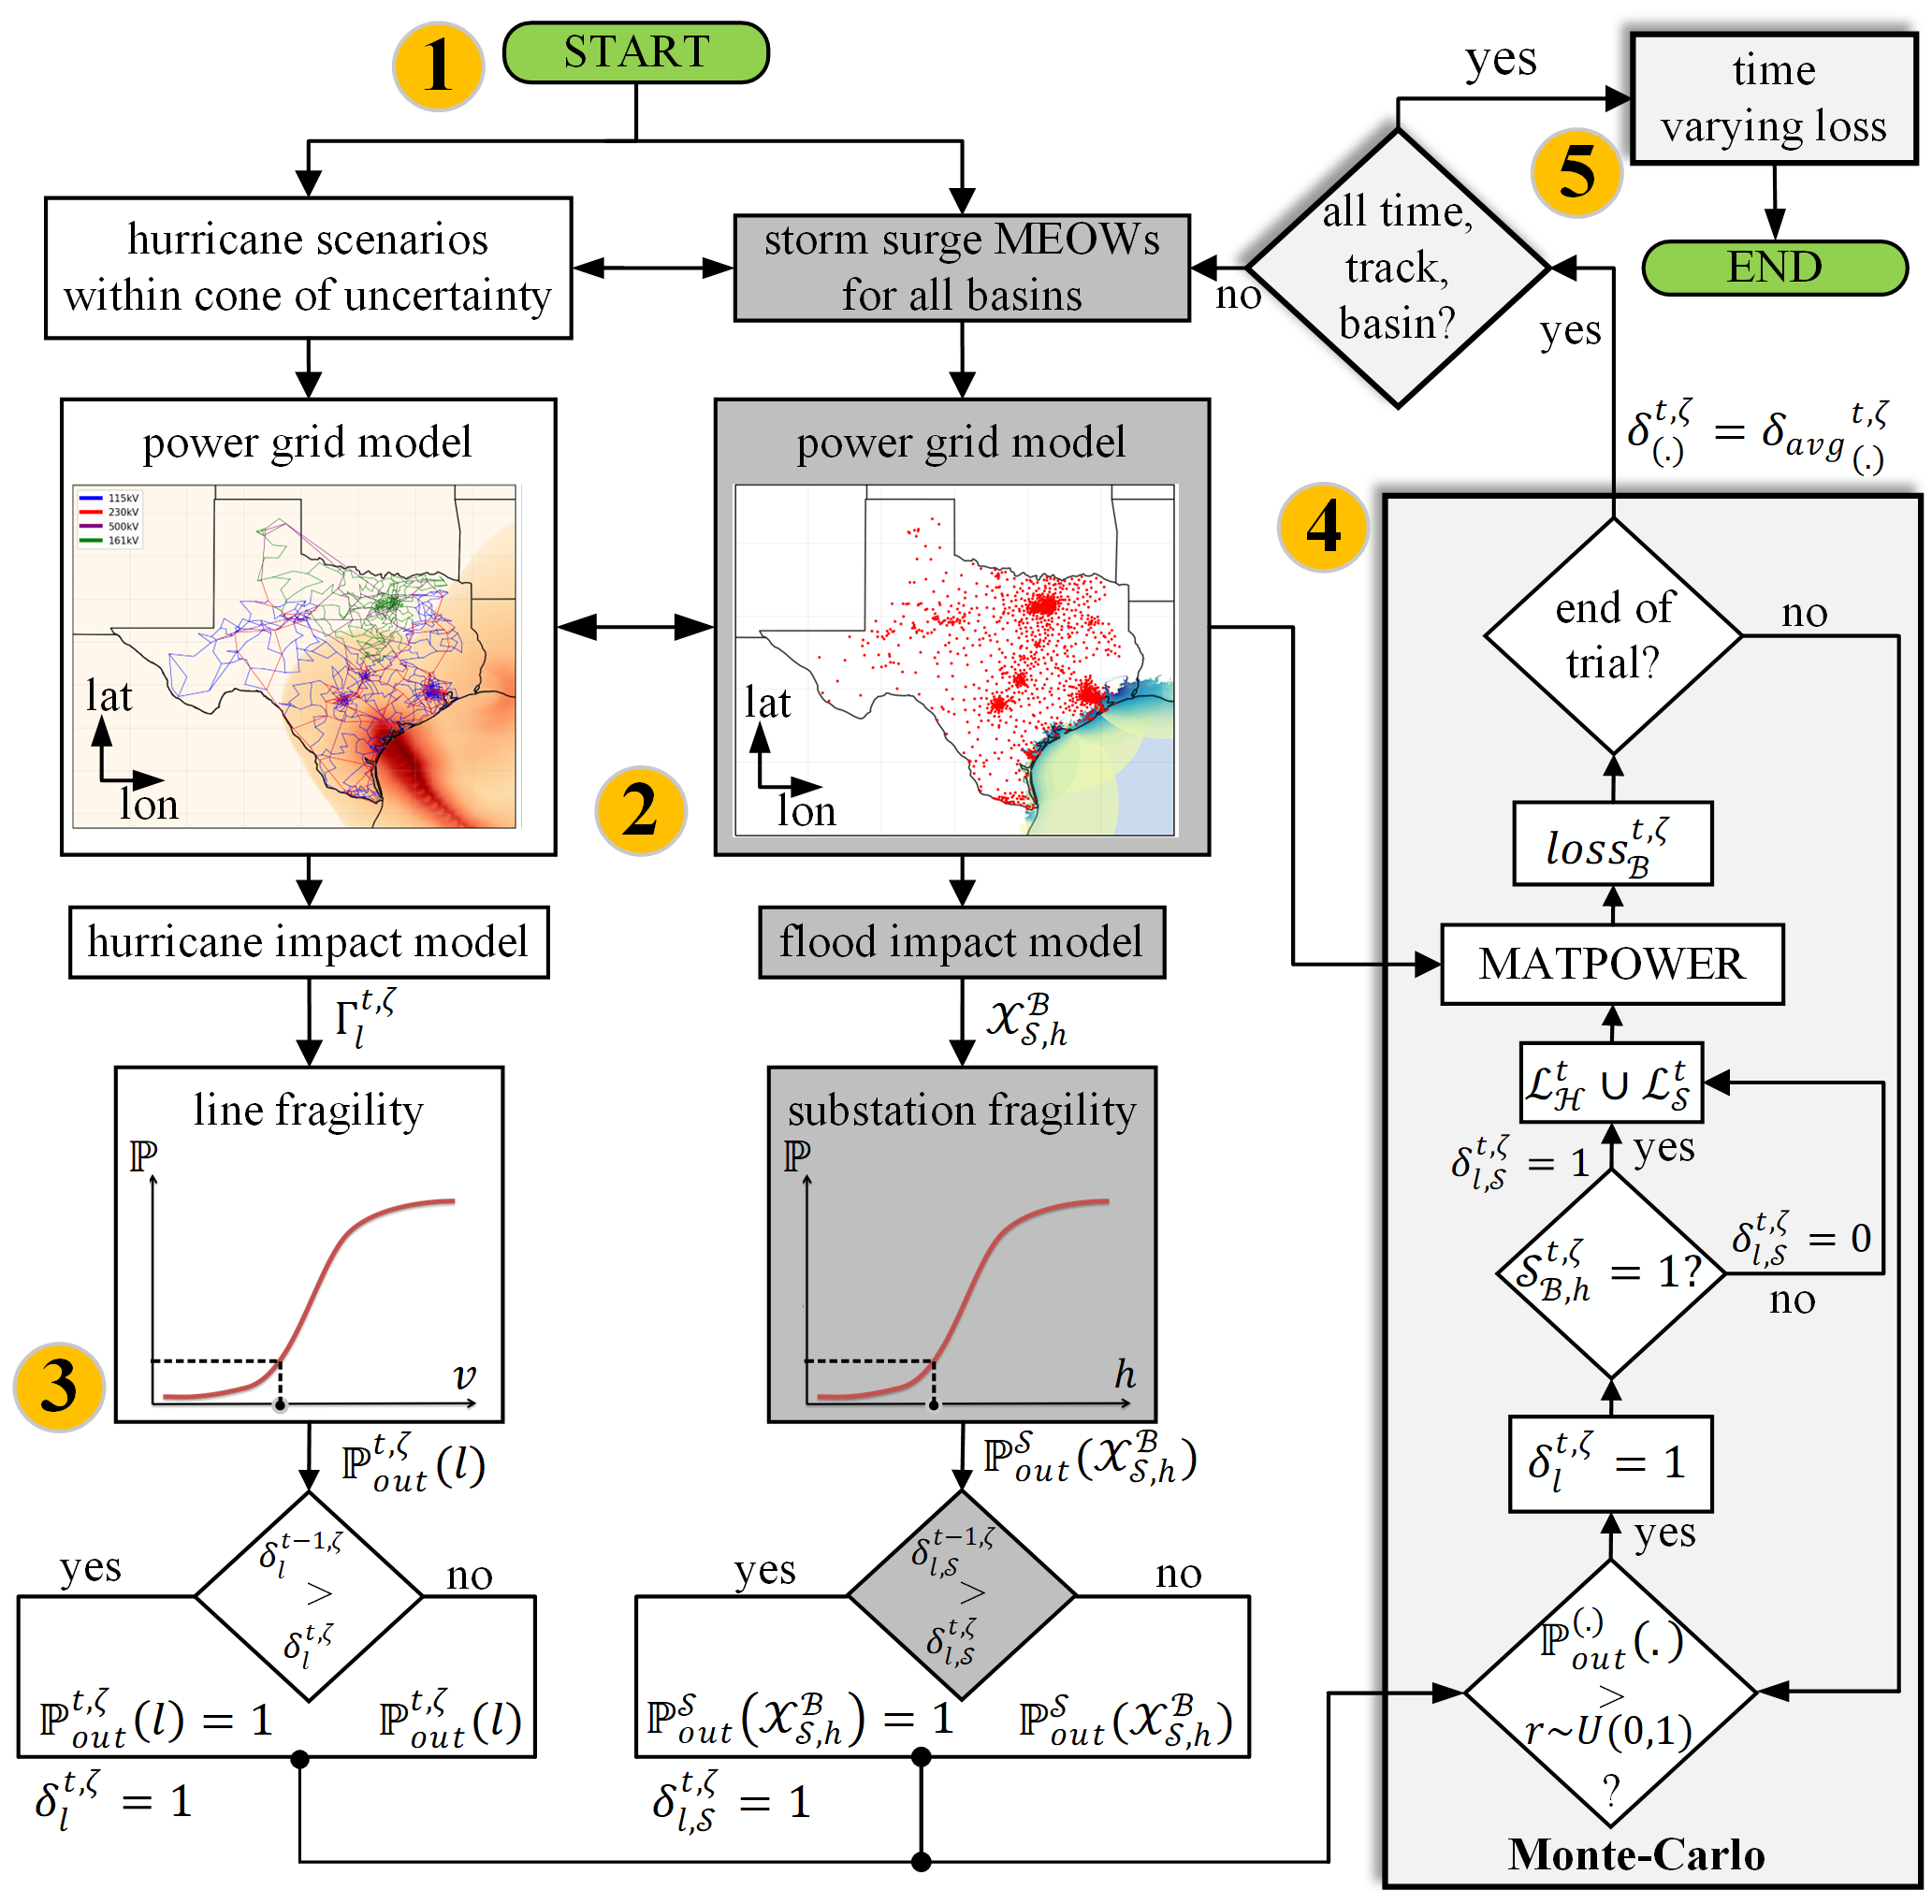
\includegraphics[width=0.7\textwidth]{figures/overall_framework.png}
   \caption{Overall architecture for generating hurricane and storm surge scenarios and grid impact assessment.}
    \label{fig:overall_architecture}
    \vspace{-5pt}
\end{figure}

\subsubsection{Hurricane and Storm Surge Scenario Generation}
The geographical data and parameters are obtained for Hurricane Harvey, that hit the coast of Texas in August 2017 using IBTrACS. Synthetic hurricane tracks are obtained by perturbing several characteristics of Hurricane Harvey, such as a shift in the initial point of origin, the amplitude of translational speed, bearing angle, landfall decay, etc. The synthetic tracks are obtained from the Climate adaptation (CLIMADA) tool. CLIMADA is a probabilistic natural catastrophe damage model that facilitates climate-based simulations~\cite{Climada}. CLIMADA can generate synthetic tracks in IBTrACS format based on the above perturbations. To synchronize the time steps for the entire duration of the hurricanes, the data is observed every two hours, and the hurricane wind field is generated for each $t$ using (\ref{eq:static_eq}). Fig.~\ref{fig:static_harvey} shows the synthetic tracks generated from CLIMADA, and the track with a solid line represents the actual track of Hurricane Harvey from IBTrACS. NOAA predicts that 7 out of 10 times, the estimated hurricane track is within the cone of uncertainty~\cite{NOAA_uncertainty}. Hence, five synthetic tracks are selected to be within the cone of uncertainty when forecasted over 120 hours of landfall, i.e., within 240 nmi as per~\cite{NOAA_uncertainty}.   

\begin{figure}[t]
    \centering
        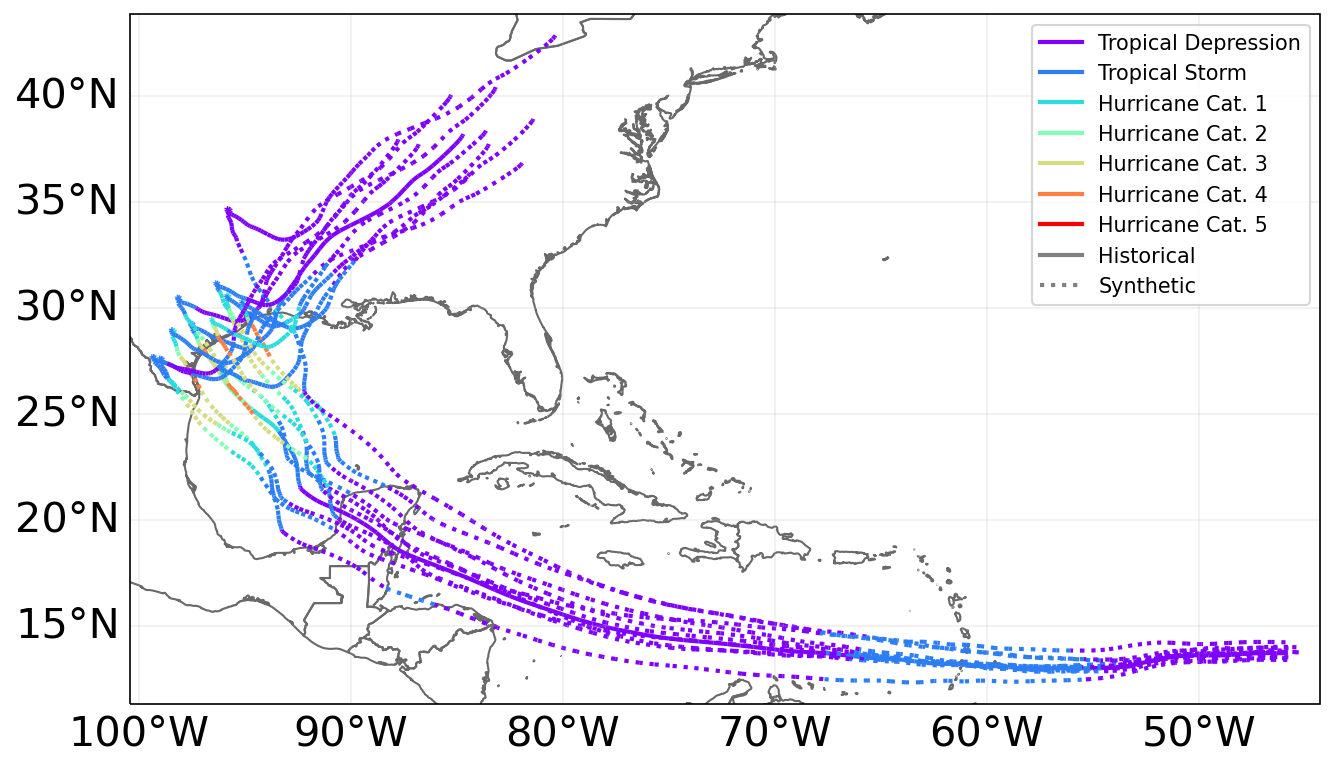
\includegraphics[width=0.7\textwidth]{figures/synthetic_tracks.png}
        \caption{Hurricane Harvey track and other synthetic tracks obtained from CLIMADA~\cite{Climada}.}
        \label{fig:static_harvey}
\end{figure}

For storm surge assessment, five different Texas basins are selected; $\mathcal{B} \in$ \{Matagorda, Corpus, Galveston, Laguna, Sabine\}. MEOW scenarios are obtained for all five basins for category 4 hurricanes moving in the northwest direction with a translational speed of 10-15 miles per hour and mean to high tide conditions. One major drawback of using MEOW maps is they are snapshots of the storm surge and carry no time information. However, we can assume that the components are not inundated until the hurricane approaches. Hence, we assign an activation flag for each component per basin at each time step. 


\subsubsection{Power Systems Impact Assessment}
This work uses a synthetic 2000-bus Texas power grid model to identify the compound probabilistic impact of hurricane and storm surges on the power grid~\cite{7725528}. The grid model maps the synthetic buses, substations, and transmission lines on the geographical footprint of Texas. There are 1250 substations and 1918 transmission lines at 4 different voltage levels --- 115 kV, 161 kV, 230 kV, and 500 kV. The total generation capacity of the system is 96291.5 megawatts (MW), and there are 1125 load units with a total size of 67109.2 MW. When the hurricane moves inland, $\Gamma_{l}^{t,\zeta}$ is obtained for each $l$ and $\mathcal{X}^\mathcal{B}_{\mathcal{S}, h}$ is obtained for each $\mathcal{S}$ from the MEOW maps. It is assumed that all substations at the coast are elevated at a level of 3 ft from the ground level. Fig.~\ref{fig:hurricane_flood_scenario} shows the wind field of Hurricane Harvey and MEOW maps on five different basins on the footprint of Texas.     

For each $\zeta$, $\mathcal{B}$, and $t$, MCS is performed for several trials. For each trial, $\mathbb{P}_{out}^{t,\zeta}(l)$ and $\mathbb{P}^{\mathcal{S}}_{out}(\mathcal{X}^\mathcal{B}_{\mathcal{S}, h})$ is compared with a uniform random number, $r\sim U(0,1)$, to identify $\mathcal{L}^t_\mathcal{H} \cup \mathcal{L}^t_\mathcal{S}$. As discussed before, MEOW maps are time-independent. However, we define an activation flag $\mathcal{S}^{t, \zeta}_{\mathcal{B}, h} \in \{0,1\}$ such that $\mathcal{S}^{t, \zeta}_{\mathcal{B},h} = 1$ makes the substation $\mathcal{S}$ inundated with depth $h$ above the ground elevation for hurricane track $\zeta$, SLOSH basin $\mathcal{B}$, and time $t$. In this work, we do not model any drainage system, and hence it is assumed that for future time steps $t+1$ the inundation level is the same. The objective here is to identify the time stamp when the substation gets flooded to analyze the compound spatiotemporal impact of two different hazards at that time step. The information, $\mathcal{L}^t_\mathcal{H} \cup \mathcal{L}^t_\mathcal{S}$, is then sent to the power grid simulator to remove the respective branches from the system. Finally, the loss for the particular $t$ is observed as the total load disconnected from the main grid. The MCS trial is conducted until the loss converges to some value.

We assume that the inundation scenarios for each $\mathcal{B}$ and each of the hurricane tracks $\zeta$ are equally likely. If $N_\zeta$ is the total number of tracks under consideration and $N_\mathcal{B}$ is the total number of basins, then the system level load loss at each time step $t$ is given by (\ref{eq:final_loss})

\begin{equation}
\small
    loss_t = \frac{1}{N_\zeta \times N_\mathcal{B}}\sum_{\zeta = 1}^{N_\zeta}{\sum_{\mathcal{B}} {loss_{\mathcal{B}}^{t,\zeta}}}
    \label{eq:final_loss}
\end{equation}

\begin{figure}[!ht!]
    \centering
    \begin{subfigure}[t]{0.7\textwidth}
        \centering
        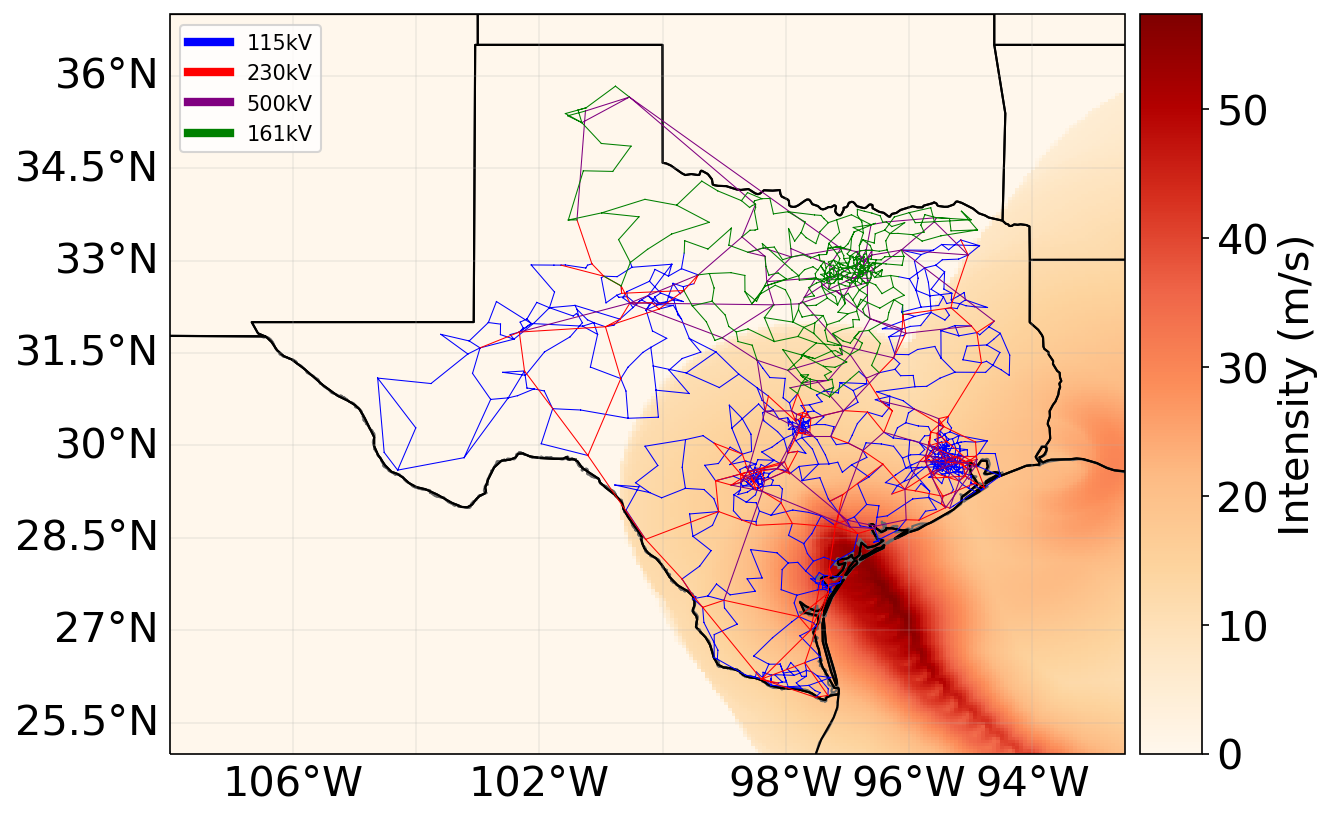
\includegraphics[width=0.8\linewidth]{figures/windfield_harvey_climada.png}
        \caption{}
        \label{fig:dynamic_harvey}
        % \vspace{-5pt}
    \end{subfigure}
    \begin{subfigure}[t]{0.7\textwidth}
        \centering
        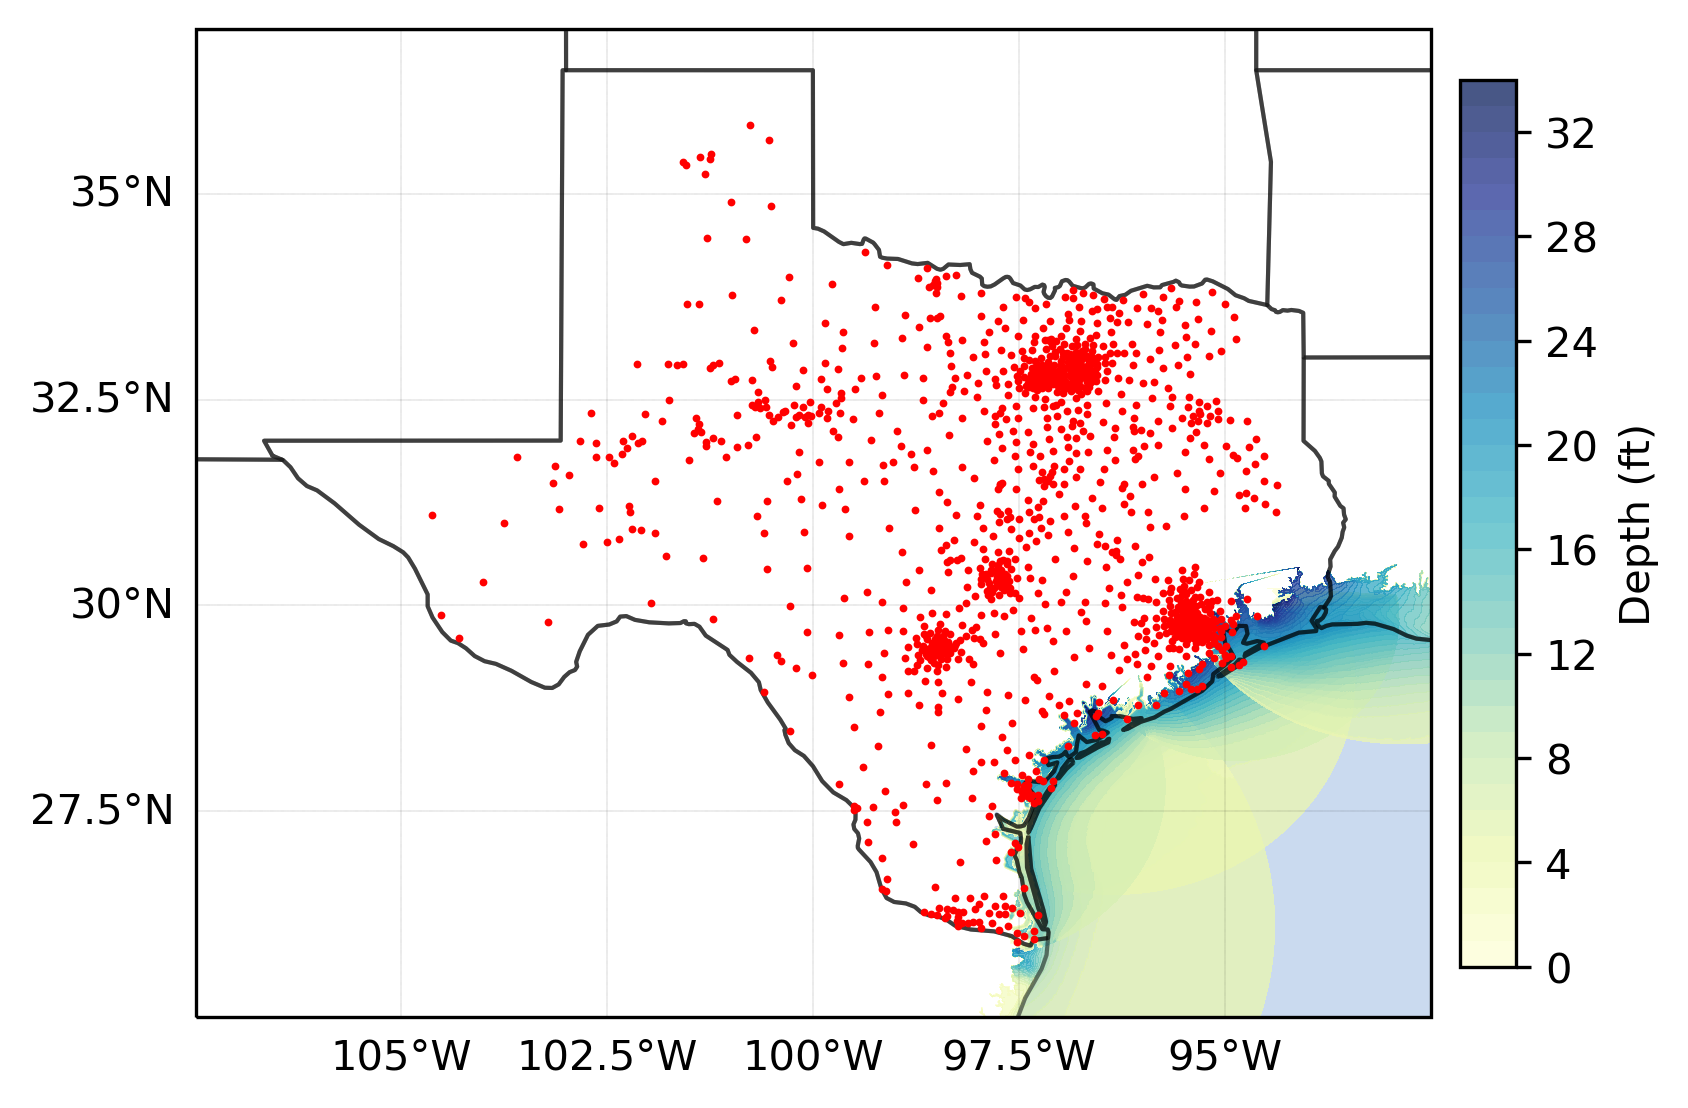
\includegraphics[width=0.8\linewidth]{figures/sub_flood.png}
        \caption{}
        \label{fig:flood_scenario}
        % \vspace{-5pt}
    \end{subfigure}
    \caption{a) Wind field of Hurricane Harvey and b) Substation flooding scenario, above ground level, for Texas basins.} 
    \label{fig:hurricane_flood_scenario}
\end{figure}

\subsection{Preliminary Research Results}
The hurricane data is obtained from IBTrACS~\cite{Knapp2010}, and synthetic hurricanes are generated using CLIMADA~\cite{Climada} in Python. SDP~\cite{SDP} is used to obtain the MEOW maps for Texas basins. The power grid is modeled in MATPOWER 7.1~\cite{5491276}, and MCS on the power grid model is conducted in MATLAB R2021a.  
From the IBTrACS, the hurricane's initial location is in the North Atlantic Ocean, which is observed at $``2017-08-16~06:00:00''$ and hence creates no impact on the power grid. Thus, the simulation for the impact assessment begins at the $100^{th}$ time step, i.e., at the advisory of $``2017-08-24~12:00:00''$. To avoid any confusion, this timestamp is referred to as $t=0$ hours for the rest of the paper. Fig.~\ref{fig:line_outage_probability} shows the outage probability of a set of transmission lines due to the original Hurricane Harvey track. It can be observed that with the moving nature and intensity of the hurricane, the outage probability of each line changes. The probability is maximum when the line experiences wind speed closer to $v_{col}$ and gradually decreases as the hurricane decays while moving inland. Fig.~\ref{fig:substation_outage_probability} represents the outage probability of substations for five different Texas basins. It is seen that the substation's vulnerability depends on the location and basin.

\begin{figure}[!h!]
    \centering
    \begin{subfigure}[t]{0.47\textwidth}
        \centering
        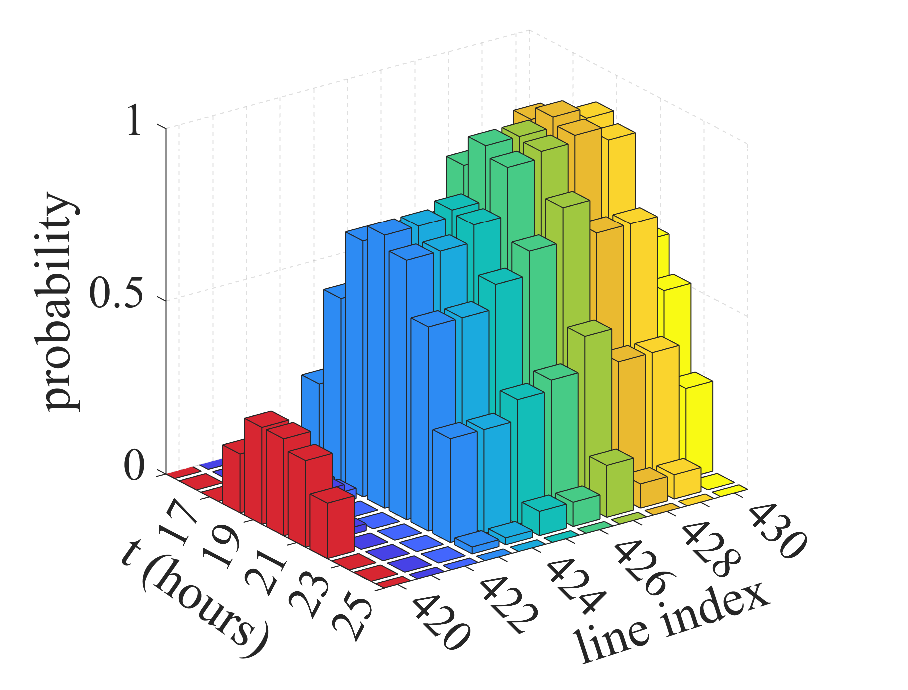
\includegraphics[width=\linewidth]{figures/outage_probability_line_.eps}
        \caption{}
        \label{fig:line_outage_probability}    
    \end{subfigure}
    \hspace*{\fill}
    \begin{subfigure}[t]{0.47\textwidth}
        \centering
        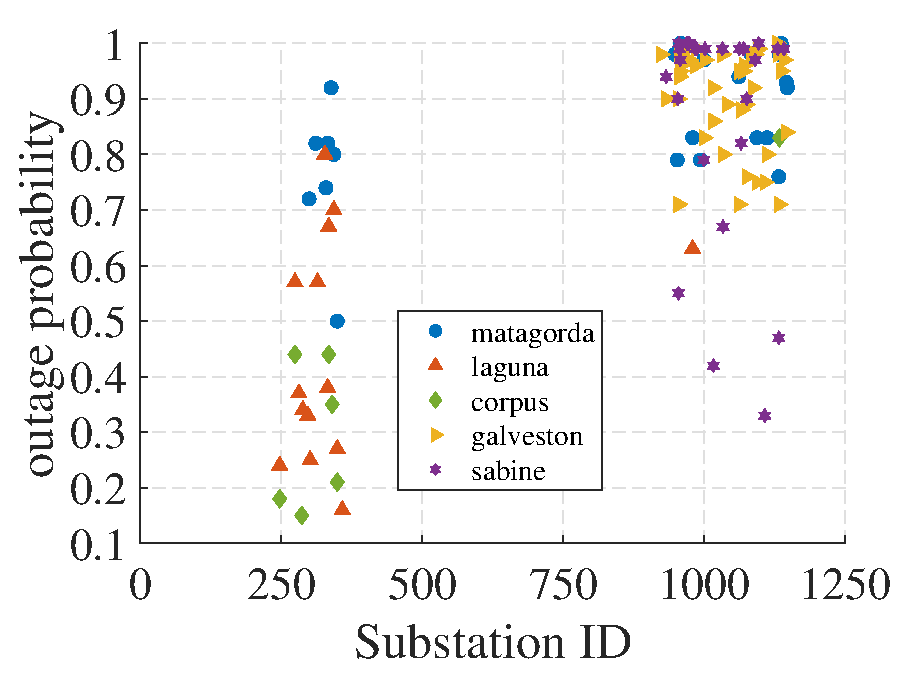
\includegraphics[width=\linewidth]{figures/outage_probability_substation_.eps}
        \caption{}
        \label{fig:substation_outage_probability}
    \end{subfigure}
    \caption{a) Line outage probability for selected lines and the original Harvey's track. b) Substation outage probability for all storm surge scenarios.} 
    \vspace{-10pt}
    \label{fig:hurricane_flood_outages}
\end{figure}

It was found that 800 Monte Carlo trials are enough to achieve convergence for any simulation case~\cite{9917119}. Hence, for each $\zeta$, $\mathcal{B}$, and $t$, 800 Monte Carlo trials are conducted. Fig.~\ref{fig:hurricane_flood_compound} shows the comparison of losses when considering the impact of the hurricane alone with the compound effect of the hurricane and the coastal flood for $\zeta=1$. It can be observed that considering substation flooding scenarios incur an additional loss of $250~MW$ by $t=50$ hours due to substation outages.   

\begin{figure}
    \centering
    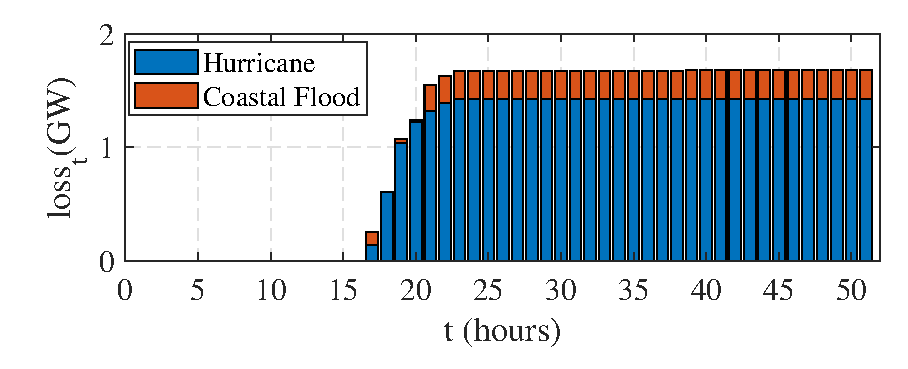
\includegraphics[width=0.7\textwidth]{figures/hurricanevsflood.eps}
    \caption{Overall loss comparison between the impact of hurricane alone and the compound impact of the hurricane and coastal flood for $\zeta = 1$.}
    \label{fig:hurricane_flood_compound}
\end{figure}

Fig.~\ref{fig:final_losses} represents the spatiotemporal loss for the compound impact of hurricane and storm surge. The dashed curves represent the loss for all basins for each track, whereas the solid blue curve represents $loss_t$ obtained from (\ref{eq:final_loss}). The loss is not incurred until $t=12$ for any $\zeta$ under consideration, and the increase is significant once the hurricane moves inland, followed by the compounded impact of storm surge. The loss increases from $loss_{12} = 9.4072$ MW to $loss_{22} = 5536.1$ MW before saturating at $loss_{40} = 6761.97$ MW as the intensity of the extreme events decreases.  

\begin{figure}[!h!]
    \centering
    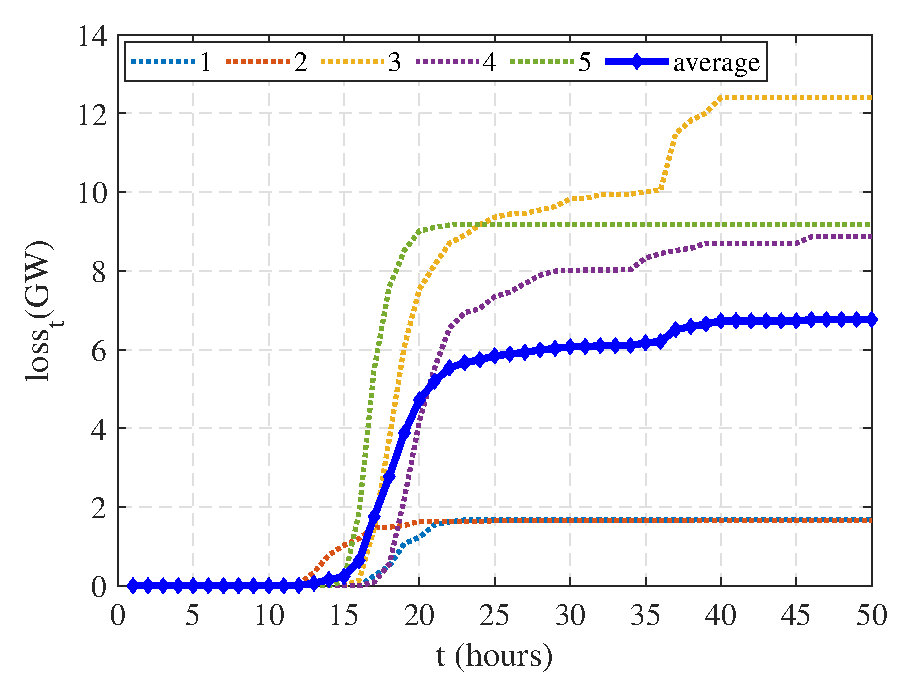
\includegraphics[width=0.7\textwidth]{figures/all_basin_losses.eps}
    \caption{Time-varying loss for each hurricane track. For each track, the loss at each time step also includes the expected value of loss over entire flood basins.}
    \label{fig:final_losses}
\end{figure}

\clearpage
% \newpage
\section{Future Works}\label{sec:future_Work}
The current work in progress aims at scaling the current resilience planning framework to solve large-scale optimization model in terms of resources, network, and scenario under consideration. As discussed in our existing work, the scenarios are time and space varying and hence such details are necessary to be incorporated in the planning model for better accuracy. Additionally, solving the extensive form of the problem is suffered by the curse of dimensionality. Hence, off-the-shelf solvers are more likely to crash or provide high optimality gap solutions when high dimensionalo extensive form of the model is fed to the solvers. Thus, solving a large-scale stochastic optimization problem has several challenges and is an active area of research that motivates us in our future work. In addition, operational planning strategies like defensive islanding would be studied to better prepare with the upcoming hurricane storms. Such proactive islanding method can prevent the propagation of cascading failure effects in the power system.

\subsection{Large-scale Resilience Planning Framework}
\subsubsection{Multiple-resource Resilience Planning using Scenario-based Dual Decomposition}
Our existing planning model plans for the DG siting and sizing problem for a range of stochastic wind events. However, the infrastructures planning problem can have multiple portfolio of resources including remote-controlled switches (RCS) and line hardening measures. There are existing works using several other planning measures as such~\cite{7514755}. However, as discussed earlier, such methods plan for the expected events but not for HILP events. The objective of this task is to formulate a planning model with multiple resources and observe the trade-off of planning among these multiple resources considering budget constraints. A dual decomposition-based algorithm will be studied to solve the scenario-based sub-problems in parallel by leveraging high-performance computing (HPC) platforms. Although such algorithms are heuristically driven, several convergence  and bounding guarantees exist in the literature for such algorithms~\cite{boland2018combining}.   

\subsubsection{Hub and Spoke Architecture for Scalable and Parallel Implementation of Stochastic Optimization}
Although parallel algorithms are faster in solving the stochastic optimization problem they can run into bottlenecks when individual sub-problems are hard to solve. In such a case, communication overhead can outweigh the parallel speedup. Such problems can rather take more time than serial methods as subproblems that have finished their work need to wait for other subproblems that have not. Hence, the objective of this task is to explore asynchronous parallel algorithm based on hub and spoke architecture as suggested in~\cite{knueven2020parallel}. When solved in hub and spoke architecture, the problems can be independently solved with less or no communication. This asynchronous problem-solving behavior increases the parallel speedup significantly. 

\subsection{Defensive Islanding and Restoration of Electric Power Systems Against Extreme Weather Events}
Extreme weather event, such as hurricane and storm surge, can have devastating impacts on the power grid and can result in cascading failures of the resources if not handled properly. During an upcoming storm, it is typically difficult to address the operational decisions considering the timescale of the events and resources required. However, it is possible to minimize the impact of these events if the grid is splitted into multiple self-sustaining islands ahead of the event. There are some existing works proposing the idea of defensive islanding. However, the event scenarios in these works are non-realistic as the spatiotemporal impact of these events are not considered. The aim of this work is to propose a defensive islanding strategy to minimize the spatiotemporal impact of extreme weather events. Furthermore, restorative actions will also be implemented once the event settles after some time.    

%\begin{comment}
\clearpage
\subsection{Timeline}
